%TC:ignore
\newcommand{\MainCiteHaagerupSzollosi}{%
  ~\cite{Haagerup1997,Szollosi2012FourParameter}}
\newcommand{\MainCiteSzollosi}{~\cite{Szollosi2012FourParameter}}
\newcommand{\MainCiteBasu}{~\cite{BasuPollackRoy2006}}
\newcommand{\MainCiteBondal}{~\cite{BondalZhdanovskiy2016}}

\title{A Complete Classification of Complex Hadamard Matrices of Order Six}

\author{Mateo C\'ardenes Wuttig}
\thanks{Contact author: \href{mailto:mateo.cardeneswuttig@yale.edu}%
{mateo.cardeneswuttig@yale.edu}}
\affiliation{Department of Applied Physics, Yale University, New Haven, Connecticut 06520, USA}
\affiliation{Yale Quantum Institute, Yale University, New Haven, Connecticut 06520, USA}
\author{Joseph Tindall}
\affiliation{Center for Computational Quantum Physics, The Flatiron Institute, 162 5th Avenue, New York, New York 10010, USA}

\ifdefined\SupplementOnly
\maketitle
%%
\tableofcontents
\clearpage
%%
\hypertarget{main-article-numbering}{}
\else
\begin{abstract}
Complex Hadamard matrices encode perfectly balanced unitary transformations.
Their classification is complete through order five, but order six -- the first dimension in which several continuous families coexist with an isolated solution -- has remained open for decades. Here, we give a complete and exact finite-incidence classification of order-six complex Hadamard matrices up to standard equivalence.
We supply the global step missing from Sz\"oll\H{o}si's dilation method, which allows us to prove an even stronger version of his conjecture: every complex Hadamard matrix of order six can be recovered algebraically from a suitable, dephased $3 \times 3$ corner defined by four initial phases.
We then describe the geometry of the reconstruction from these phases and show that, except for Tao's isolated matrix and a single explicit Karlsson matrix, every class admits a representative obtained by solving one quadratic and one cubic equation in both the horizontal and vertical directions.
Our work resolves the classification problem and provides a rigorous framework for further investigating order-six Hadamards, with applications to balanced six-mode interferometers and the study of mutually unbiased bases.
\end{abstract}
\maketitle

\section{Introduction}
Complex Hadamard matrices are square matrices with entries of unit magnitude and mutually orthogonal rows. They arise directly in quantum mechanics as equal-amplitude unitary changes of basis. The subject grew from Sylvester's constructions and Hadamard's determinant problem for real sign matrices with orthogonal rows~\cite{Sylvester1867,Hadamard1893}. 

A physical realization of complex Hadamards is provided by multimode quantum interferometry. After normalization, an order-six complex Hadamard matrix is a perfectly balanced six-port unitary, with identical single-particle transition probabilities but generally different multiparticle interference determined by its internal phases~\cite{Carolan2015Universal,Laing2012BerryPhase,Tichy2010ZeroTransmission,Crespi2015Sylvester,Crespi2016FFT,Shchesnovich2015Partial}. Complex Hadamards are also utilized as coherence-generating gates~\cite{Yao2016MaximalCoherence}, mixing operations in quantum walks~\cite{Mackay2002QuantumWalks,Lorz2019PhotonicWalks}, elements of dual-unitary dynamics~\cite{Gutkin2020DualUnitary,Claeys2022StateDesigns}, and as core components in teleportation, error correction, and contextuality protocols~\cite{Werner2001Teleportation,Musto2016QuantumLatin,Lisonek2019KochenSpecker}. 

Complex Hadamards are also intimately involved in the study of mutually unbiased bases. Two orthonormal bases $\{e_j\}$ and $\{f_k\}$ of the complex Hilbert space $\C^d$ are mutually unbiased when $|\langle e_j,f_k\rangle|=1/\sqrt d$ for every $j,k$. After one basis is
chosen as the standard basis, multiplying the transition matrix to the other basis by $\sqrt d$ gives a complex Hadamard matrix~\cite{TadejZyczkowski2006,WoottersFields1989,BengtssonEtAl2007}.
Determining how many mutually unbiased bases exist in $\C^6$ is one of the central open problems of quantum information theory~\cite{HorodeckiRudnickiZyczkowski2022,McNultyWeigert2026,BengtssonEtAl2007,MatolcsiEtAl2026MUBTriplets}. A complete classification of the $d =6$ Hadamards would provide a natural framework for addressing this problem.

The classification of all complex Hadamard matrices is complete through order five. In dimensions $d=2,3$ and $5$, they are fully classified by the Fourier matrix, while in $d=4$ there is, up to standard equivalence, one continuous one-parameter family~\cite{Haagerup1997,TadejZyczkowski2006}.
Order six is the first, until now, unresolved case, and it is also the first order at which several inequivalent continuous families coexist with a genuinely isolated matrix~\cite{TadejZyczkowski2006,Szollosi2012FourParameter,BengtssonEtAl2007,Tadej2008}. The introduction of Sz\"oll\H{o}si's dilation algorithm~\cite{Szollosi2012FourParameter} represents a significant milestone in the study of order six. The algorithm starts with a dephased $3\times3$ corner of the full matrix, finds candidate blocks completing its first three rows and columns, and then forces the remaining block by linear algebra. Sz\"oll\H{o}si proved that this procedure is exhaustive for a fixed corner when the normalized candidate sets of invertible blocks are finite~\cite{Szollosi2012FourParameter}. He conjectured that, apart from Karlsson's family~\cite{Karlsson2011H2,Karlsson2011ThreeParameter} and Tao's isolated 
matrix~\cite{Tao2004,BengtssonEtAl2007,Tadej2008}, every order-six complex Hadamard could be recovered in this way. 
Bondal and Zhdanovskiy later proved the existence of a family of order-six complex Hadamard matrices of real dimension four~\cite{BondalZhdanovskiy2016}. More recently, several special subclasses have been studied, including non-$H_2$-reducible examples, matrices with prescribed column patterns, eigenvalue-constrained two-parameter families, and matrices with exactly three distinct entries~\cite{LiangEtAl2024,MatszangoszSzollosi2024,HuangChen2026Eigenvalues,HuangLiangChen2026ThreeElements}.
%


Two obstacles remained between Sz\"oll\H{o}si's fixed-corner result~\cite{Szollosi2012FourParameter} and a complete classification.
First, Sz\"oll\H{o}si's published formulas use divisions and generic polynomial degrees, so special finite branches require separate care.
Second, a chosen corner may have infinitely many candidate blocks that complete it, so fixed-corner completeness does not guarantee that every matrix has a finite corner.

In this work, we close both gaps. We solve exactly for every normalized side block compatible with the chosen corner, using division-free equations so that valid solutions on vanishing-denominator branches are not lost. We then prove that every order-six complex Hadamard matrix has at least one $3\times3$ corner with only finitely many compatible normalized side blocks. At such a corner the actual adjacent blocks occur in the finite candidate sets and the remaining block is uniquely forced. The resulting branch-complete dilation procedure is therefore sound and exhaustive, giving an exact finite-incidence classification and proving Sz\"oll\H{o}si's Conjecture~4.2~\cite{Szollosi2012FourParameter}.

The result of our branch-complete dilation procedure is an explicit classification of all order-six complex Hadamard matrices, up to standard equivalence.
Except for the equivalence classes associated with Tao's isolated matrix and a single explicit Karlsson matrix, every class is shown to admit a representative matrix with a \textit{product-regular} corner specified by just four phase parameters. 
By product-regular, we mean the matrix can be reconstructed using the four phases by solving one quadratic and one cubic equation in each of the horizontal and vertical directions. Compatible solutions determine the adjacent blocks and uniquely force the final $3\times3$ block, whose entries are automatically of unit magnitude.

This work is structured as follows. In section~\ref{sec:definition_hadamard}, we introduce complex Hadamard matrices, the Tao and Karlsson families, and outline the main ideas underlying the classification proof.
Section~\ref{sec:mainclassification} defines our branch-complete finite-dilation extension of Sz\"oll\H{o}si's algorithm before going on to prove the classification.
Section~\ref{sec:atlas} studies the resulting reconstruction over the four-phase seed torus, introducing the notion of product regularity, the corresponding physical domain over the four seed space and relates this local geometry to the full class space.
Section~~\ref{sec:szollosi-conjecture} defines the output of Sz\"oll\H{o}si's published fixed-corner construction and utilizes our classification theorem to prove his conjecture that every order-six class outside the Karlsson and Tao sectors can be recovered by his fixed-corner construction.
In section~\ref{sec:outlook} we conclude by discussing the implications of this classification for the geometry of the order-six Hadamard space, mutually unbiased bases, multiphoton interferometry, and related applications in quantum information and quantum dynamics.
The Supplemental Material~\cite{SupplementalMaterial} contains the complete technical proofs. An accompanying Lean~4 formalization independently verifies the complete classification without relying on any previous classification results~\cite{deMouraUllrich2021,CardenesWuttig2026HadamardRepository}. The separate four-phase geometry of Sec.~\ref{sec:atlas} is supported by exact certificates in the same Github repository~\cite{CardenesWuttig2026HadamardRepository}.

\section{Complex Hadamard Matrices}
\label{sec:definition_hadamard}
\begin{definition}[Complex Hadamard matrix]
\label{def:hadamard}
The unit circle in the complex plane $\C$ is defined as
\begin{equation}
\T=\{z\in\C:|z|=1\}.
\label{eq:unitcircle}
\end{equation}
For $m\geq1$, the torus
\begin{equation}
    \T^m=\{(z_1,\ldots,z_m)\in\C^m:|z_j|=1\ \text{for all }j\},
\end{equation}
is the space of $m$ independent phases. 
A matrix is called unimodular if all of its entries lie in $\T$.
A complex Hadamard matrix of order $n$ is a matrix
$H\in\T^{n\times n}$ satisfying
\begin{equation}
HH^{\dagger}=nI_n,
\label{eq:hadamarddef}
\end{equation}
where $H^{\dagger}$ is the conjugate transpose and $I_n$ is the identity matrix of order $n$. Since $H$ is square, Eq.~\eqref{eq:hadamarddef} is equivalent to
$H^{\dagger}H=nI_n$~\cite{TadejZyczkowski2006}.
\end{definition}

\begin{definition}[Standard equivalence and the class space]
\label{def:equivalence}
Two order-$n$ complex Hadamard matrices are equivalent, written $H\sim H'$, if diagonal unitary matrices $D_{\rm r},D_{\rm c}$ and permutation matrices $P_{\rm r},P_{\rm c}$ exist such that
\begin{equation}
H'=D_{\rm r}P_{\rm r}HP_{\rm c}D_{\rm c}.
\label{eq:equivalence}
\end{equation}
The equivalence class of $H$ is written as $[H]=\{H':H'\sim H\}$. 
A matrix is called dephased if every entry of its first row and first column equals $1$. Every equivalence class contains a dephased representative. 
For a fixed row and column ordering, dephasing produces a unique matrix~\cite{TadejZyczkowski2006,Szollosi2012FourParameter}.
We define the order-six class space by
\begin{equation}
\HH_6 =\bigl\{[H]:H\in\T^{6\times6},\ HH^{\dagger}=6I_6\bigr\}.
\label{eq:H6classes}
\end{equation}
\end{definition}

\begin{definition}[Fourier matrix]
\label{def:fouriermatrix}
The Fourier matrix $F_n$ is a complex Hadamard matrix which exists for every order $n$, defined through its entries
\begin{equation}
(F_n)_{jk}=\exp\!\left(\frac{2\pi\I jk}{n}\right),
\qquad 0\leq j,k<n
\label{eq:fouriern}
\end{equation}
where $\I$ denotes the imaginary unit,
$\I^2=-1$. 
\end{definition}

A $k$-parameter family is a set of equivalence classes
\begin{equation}
\mathcal F_k=\{[H(\mathbf z)]:\mathbf z=(z_1,\ldots,z_k)\in\T^k\}
\subseteq\HH_6,
\end{equation}
where the $k$ phases are independent real coordinates.
%
In dimension six, Di\c{t}\u{a}-type, circulant, self-adjoint, and other structured ansätze form important continuous families~\cite{Dita2004,BeauchampNicoara2008,MatolcsiSzollosi2008,
Szollosi2010Hypocycloids}. 
Karlsson proved that every matrix containing a $2\times2$ Hadamard submatrix belongs to his complete three-parameter
family~\cite{Karlsson2011H2,Karlsson2011ThreeParameter}. 
%
We first define the Karlsson family intrinsically through reducibility to order two Hadamard matrices $H_2$.
\begin{definition}[$2\times2$ Hadamard submatrix]
A $2\times2$ complex Hadamard submatrix is any choice of two rows and two columns whose intersection is itself a $2\times2$ complex Hadamard matrix. An order-six complex Hadamard matrix is $H_2$-reducible if it is equivalent to a matrix with such a submatrix. Equivalently, allowed row and column operations can expose the
canonical block
\begin{equation}
F_2=\begin{pmatrix}1&1\\1&-1\end{pmatrix}.
\label{eq:F2}
\end{equation}
We define the Karlsson sector by
\begin{equation}
    \KK_6^{(3)}=\{[H]\in\HH_6:H\text{ is }H_2\text{-reducible}\}.
\label{eq:karlsson}
\end{equation}
Karlsson's theorem identifies this set exactly with the equivalence classes generated by his explicit three-real-parameter family
~\cite{Karlsson2011H2,Karlsson2011ThreeParameter}.
\end{definition}

%%%%%%%%%%%%%%%%%%%%
% Move around
\begin{figure}[htb!]
\centering
\begingroup
\begin{tikzpicture}[
  every node/.style={font=\footnotesize,align=center},
  >={Latex[length=1.9mm,width=1.25mm]},
  flow/.style={->,semithick,draw=black!62,rounded corners=2pt},
  full/.style={rounded corners=2pt,inner xsep=5pt,inner ysep=3pt,
               minimum width=.90\columnwidth,text width=.82\columnwidth},
  decision/.style={full,draw=black!45,densely dashed,fill=black!1},
  neutral/.style={full,draw=black!42,fill=black!2},
  bluebox/.style={full,draw=blue!58!black,fill=blue!3},
  output/.style={full,draw=blue!68!black,thick,fill=blue!4},
  edge/.style={font=\scriptsize,fill=white,inner sep=1pt,text=black!62},
  panel/.style={font=\footnotesize\bfseries,text=black,inner sep=0pt,outer sep=0pt},
  classlabel/.style={font=\footnotesize,align=center,text=black},
  eqsymbol/.style={font=\footnotesize,align=center,text=black,inner sep=0pt,outer sep=0pt},
  disjoint/.style={font=\normalsize,align=center,text=black,inner sep=0pt,outer sep=0pt},
  pregion/.style={draw=black!75,fill=cyan!8,rounded corners=4pt,
                  minimum width=.575\columnwidth,minimum height=10.0mm},
  subclass/.style={classlabel,draw=black!70,fill=violet!9,rounded corners=3pt,
                   minimum height=6.1mm},
  isolated/.style={circle,draw=black!75,fill=red!8,minimum size=9.4mm,
                   inner sep=0pt,outer sep=0pt}
]

% (a) Proof architecture: only the main logical spine is shown here.
\node[decision] (choice) {%
  \textbf{Finite-corner search}\\[-1pt]
  For arbitrary $[H]\in\HH_6$, inspect all $400$\\[-1pt]
  positional corners.\\[-1pt]
  \emph{Is any selected $3\times3$ corner a finite-corner witness?}%
};
% The left boundary includes the outer ``yes'' branch.
\coordinate (figleft) at ([xshift=-7.2mm]choice.west);
\node[panel,anchor=south west]
  at ($(figleft |- choice.north)+(0,0.8mm)$) {\textbf{A.}};

\node[neutral,below=4.4mm of choice] (routing) {%
  \textbf{Failure-of-search route}\\[-1pt]
  \hyperref[prop:main-infinite-fiber-trichotomy]{Propositions.~\ref*{prop:main-infinite-fiber-trichotomy}--\ref*{thm:finitecornerintro}},
  \hyperref[prop:karlsson-finite-corner]{\ref*{prop:karlsson-finite-corner}},
  \hyperref[prop:tao-finite-corner]{\ref*{prop:tao-finite-corner}}\\[-1pt]
  If every test fails, $[H]\in\KK_6^{(3)}$ or $\mathcal T_6$;\\[-1pt]
  both sectors provide a finite-corner witness.%
};

\node[bluebox,below=4.4mm of routing] (witness) {%
  \textbf{Universal finite-corner theorem}\\[-1pt]
  \hyperref[thm:classification]{Theorem~\ref*{thm:classification}}\\[-1pt]
  Every $[H]\in\HH_6$ has a finite-corner witness.%
};

\node[bluebox,below=4.4mm of witness] (dilation) {%
  \textbf{Branch-complete dilation}\\[-1pt]
  \hyperref[prop:algorithmvalid]{Proposition~\ref*{prop:algorithmvalid}}\\[-1pt]
  The finite candidate lists reconstruct $H$.%
};

\node[output,below=4.4mm of dilation] (finish) {%
  \textbf{Exact retained output}\\[-1pt]
  \hyperref[cor:atlas-classification]{Corollary~\ref*{cor:atlas-classification}}\\[-1pt]
  $\FCAtlas_6^{\mathrm{fc}}=\HH_6$%
};

\draw[flow] (choice.south)
  -- node[edge,right,midway,xshift=1.2mm,font=\footnotesize] {no}
  (routing.north);
\draw[flow] (choice.west)
  -- ++(-4.0mm,0)
  node[edge,above,pos=.45,xshift=-1.0mm,font=\footnotesize] {yes}
  -- (figleft) |- (witness.west);
\draw[flow] (routing.south) -- (witness.north);
\draw[flow] (witness.south) -- (dilation.north);
\draw[flow] (dilation.south) -- (finish.north);

% (b) Class-space structure
\coordinate (brow) at ([yshift=-11.0mm]finish.south);
\node[panel,anchor=west] (panelb)
  at (figleft |- brow) {\textbf{B.}};
\node[eqsymbol,anchor=west] (hclass)
  at ([xshift=3.2mm]finish.west |- brow) {$\HH_6$};
\node[eqsymbol,anchor=west] (equals)
  at ([xshift=0.9mm]hclass.east |- brow) {$=$};
\node[pregion,minimum width=.38\columnwidth,anchor=west] (preg)
  at ([xshift=0.9mm]equals.east |- brow) {};
\coordinate (pregrow) at (preg.center);
\node[subclass,minimum width=.245\columnwidth,anchor=east] (kclass)
  at ([xshift=-2.5mm]preg.east |- pregrow)
  {$\KK_6^{(3)}\setminus\{[H_\times]\}$};
\coordinate (pcenter) at ($($(preg.west)!0.5!(kclass.west)$ |- pregrow)$);
\node[classlabel,anchor=center] at (pcenter) {$\mathcal P_6$};
\node[disjoint,anchor=west] (unionone)
  at ([xshift=1.9mm]preg.east |- brow) {$\mathbin{\dot\cup}$};
\node[isolated,anchor=west] (taoclass)
  at ([xshift=1.9mm]unionone.east |- brow) {};
\node[classlabel] at (taoclass.center) {$\mathcal T_6$};
\node[disjoint,anchor=west] (uniontwo)
  at ([xshift=1.9mm]taoclass.east |- brow) {$\mathbin{\dot\cup}$};
\node[isolated,anchor=west] (hxclass)
  at ([xshift=1.9mm]uniontwo.east |- brow) {};
\node[classlabel] at (hxclass.center) {$\{[H_\times]\}$};
\end{tikzpicture}
\vspace{2pt}
\caption{\textbf{Proof architecture and class-space structure.} \textbf{A.} Choose three rows and three columns of $H=\left(\begin{smallmatrix}E&B\\ C&D\end{smallmatrix}\right)\in\T^{6\times6}$, move the selected $3\times3$ block to the upper-left position, dephase, and write its four free entries as $(a,b,c,d)\in\T^4$. For each of the $\binom{6}{3}^{2}=400$ positional choices, the normalized invertible horizontal and vertical candidate sets adjacent to $E$ are denoted by $\mathcal B_E^{\times}$ and $\mathcal C_E^{\times}$. A finite-corner witness is a corner for which both sets are nonempty and finite and contain the actual adjacent blocks $B$ and $C$, respectively (\hyperref[def:finitecorner]{Definition~\ref*{def:finitecorner}}). At a successful corner, Sz\"oll\H{o}si's fixed-corner construction applies. If every test fails, the failure-of-search route places $H$ in the Karlsson or Tao sector, where finite-corner witnesses are produced, proving the universal finite-corner theorem. At the witnessing corner, the branch-complete procedure extends Sz\"oll\H{o}si's Construction~3.1~\cite{Szollosi2012FourParameter} by retaining the uncancelled fixed-Gram systems on exceptional branches, the actual $B,C$ occur in the finite candidate lists, and the uniquely forced block $D=-CE^\dagger(B^{-1})^\dagger$ reconstructs $H$. \hyperref[def:completed-output]{Definition~\ref*{def:completed-output}} specifies the completed output. \textbf{B.} $\HH_6$ is the full class space of all order-six complex Hadamard matrices. The product-regular set $\mathcal P_6$, defined in \hyperref[subsec:global-reach-regular-cover]{Sec.~\ref*{subsec:global-reach-regular-cover}}, contains the product-regular Karlsson classes $\KK_6^{(3)}\setminus\{[H_\times]\}$. \hyperref[thm:global-product-regular-escape]{Theorem~\ref*{thm:global-product-regular-escape}} identifies the two classes outside $\mathcal P_6$ as Tao's isolated class $\mathcal T_6$ and the unique product-exceptional Karlsson class $\{[H_\times]\}$.}
\label{fig:finite-corner-proof}
\endgroup
\end{figure}

%%%%%%%%%%%%%%%%%%%%

Distinct from it lies the isolated cubic-root matrix $S_6^{(0)}$ associated with Tao's work~\cite{Tao2004,TadejZyczkowski2006,Szollosi2012FourParameter,Tadej2008}. \begin{definition}[Tao's dephased matrix]
Let $\omega=\exp(2\pi\I/3)$. Then $\omega^3=1$, $\omega\ne1$, and $1+\omega+\omega^2=0$. Tao's dephased matrix~\cite{Tao2004} is
\begin{equation}
S_6^{(0)}=
\begin{pmatrix}
1&1&1&1&1&1\\
1&1&\omega&\omega&\omega^2&\omega^2\\
1&\omega&1&\omega^2&\omega^2&\omega\\
1&\omega&\omega^2&1&\omega&\omega^2\\
1&\omega^2&\omega^2&\omega&1&\omega\\
1&\omega^2&\omega&\omega^2&\omega&1
\end{pmatrix},
\label{eq:taomatrix}
\end{equation}
\end{definition}
which is complex Hadamard. We define the one-point Tao sector~\cite{Tao2004} by
\begin{equation}
\mathcal T_6=\{[S_6^{(0)}]\}.
\label{eq:Taosector}
\end{equation}

We can write any complex Hadamard matrix of order six in block form as
\begin{equation}
H=
\begin{pmatrix}
E&B\\
C&D
\end{pmatrix},
\label{eq:blockform}
\end{equation}
where $E,B,C,D\in\T^{3\times3}$. Sz\"oll\H{o}si's dilation construction~\cite{Szollosi2012FourParameter} starts from a dephased $3\times3$ corner $E$, determines the normalized candidate blocks $B$ and $C$ from their fixed-Gram constraints, and then forces $D$ by block orthogonality. We call the complete normalized solution set for $B$ or $C$ a \emph{side fiber}.

Sz\"oll\H{o}si's fixed-corner completeness theorem states that, when the two invertible side fibers of a prescribed corner $E$ are finite and nonempty, pairing all their candidates and testing the forced block $D$ enumerates every Hadamard completion containing $E$. Accordingly, a selected $3\times3$ corner of a given order-six Hadamard matrix $H$ is a \emph{finite-corner witness} if its two invertible side fibers are finite and nonempty and contain the actual adjacent blocks $B$ and $C$. The original matrix $H$ is then recovered among finitely many completions.
The fixed-corner theorem is conditional: some corners have infinite side fibers, and it does not show that every Hadamard matrix possesses a finite-corner witness. 

In the following, we prove that every order-six complex Hadamard matrix has such a witness. We show that an infinite side fiber forces either a Fourier block, a strictly negative real cubic Gram invariant, or the Karlsson sector. Outside the latter case, complementary $3\times3$ blocks reverse the sign of the cubic invariant, producing a corner with two finite side fibers unless all four complementary blocks are Hadamard. This case then reduces to the Karlsson or Tao sectors. Neither sector is excluded from the witness theorem: every Karlsson class admits a finite-corner witness, while the leading $3\times3$ corner of Tao's matrix is one. Thus every order-six complex Hadamard matrix has a finite-corner witness, closing the gap between Sz\"oll\H{o}si's fixed-corner construction and an exhaustive classification.

%%%%%%%%%%%%%%%%%%%%%%%%%%%%%%%%%%%%%%%%%%%%%%%%%%
\section{Finite-corner classification}
\label{sec:mainclassification}
%%%%%%%%%%%%%%%%%%%%%%%%%%%%%%%%%%%%%%%%%%%%%%%%%%

We formulate the classification in terms of finite $3\times3$ corners.
Choose three rows and three columns of an order-six Hadamard matrix, move them to the leading positions (rows and columns $1,...,3$), and dephase. The matrix splits into four $3\times3$ blocks as in Eq.~\eqref{eq:blockform}, and we call its upper-left block $E$ the \emph{corner} for that choice of rows and columns. Orthogonality of the full matrix fixes every inner product among the rows of the block $B$ and among the columns of the block $C$ in terms of $E$ alone. Each of $B$ and $C$ is therefore confined to a set of candidates determined by the corner (see Eq.~\eqref{eq:candidatesets}).
If both candidate sets are finite and nonempty they can be listed exhaustively, the fourth block is then determined, and the matrix we started from is recovered among the finitely many completions. Such a corner is a \emph{finite-corner witness}, defined rigorously in Definition~\ref{def:finitecorner}.

\begin{theorem}[Complete finite-corner classification]
\label{thm:classification}
Every order-six complex Hadamard matrix is equivalent to a dephased matrix
having a finite-corner witness.
\end{theorem}

Figure~\ref{fig:finite-corner-proof}(a) summarizes the proof, which is assembled at the end of this section. Below, we state two structural results from the literature used in this manuscript's proof. We emphasize that the accompanying Lean formalization ~\cite{CardenesWuttig2026HadamardRepository} directly proves the parts of both results needed for the classification, rather than using them as assumptions. We then formulate our branch-complete refinement of Sz\"oll\H{o}si's dilation construction~\cite{Szollosi2012FourParameter}, which retains solutions on branches where the divisions used in a generic implementation would be invalid.

The central step in our proof is then a global routing argument. Starting from an arbitrary order-six Hadamard matrix, we examine all $400$ positional corners. 
If none of them are a finite-corner witness, then at least one side fiber is infinite at every corner. We show that, by analyzing these infinite fibers and their complementary blocks, this forces the matrix into either the Karlsson or Tao sector. We then prove separately that every matrix in the Karlsson and Tao sectors has a finite-corner witness. 
Hence, every order-six complex Hadamard matrix has such a witness. Applying the branch-complete construction at that corner recovers the original matrix, and therefore completes the classification.
The full class space of all Hadamard matrices in sketched in Figure~\ref{fig:finite-corner-proof}(b).

\subsection{Structural results used in the universal proof}
The proof in this manuscript starts from two previously established structural results for order-six Hadamard matrices. 

\begin{proposition}[Published order-six structural inputs]
\label{prop:publishedinputs}
For an order-six complex Hadamard matrix $H$:
\begin{enumerate}
\item $H$ is $H_2$-reducible if and only if it is equivalent to a
member of Karlsson's complete three-real-parameter family
\cite{Karlsson2011H2,Karlsson2011ThreeParameter}. Karlsson's
parametrization also covers the parameter values at which both
M\"obius formulas degenerate: the resulting Hadamard matrices are,
up to equivalence, members of the two-parameter Fourier family
$F_6^{(2)}$ or its transpose
\cite[Secs.~4--5 and Theorem~11]{Karlsson2011ThreeParameter}.
See also
\cite[p.~623, Theorem~2.11]{Szollosi2012FourParameter}.
\item If $H$ is equivalent to a dephased complex Hadamard matrix having both a noninitial row and a noninitial column composed entirely of cubic roots of unity, then either $[H] \in \mathcal T_6$ or
$[H]\in\KK_6^{(3)}$~\cite[p.~624, Lemma~2.14]{Szollosi2012FourParameter}. 
In a dephased matrix, a noninitial row or
column is any other than the first.
%\footnote{The theorem and lemma numbers just cited are those of the final journal version\cite{Szollosi2012FourParameter}. The arXiv v1 numbering differs: the corresponding results are Theorem~2.12 and Lemma~2.15, with the conjecture 4.4.}
\end{enumerate}
\end{proposition}

Our accompanying Lean~4 formalization \cite{CardenesWuttig2026HadamardRepository} does not assume the two published results of Proposition~\ref{prop:publishedinputs}. It proves both within Lean as part of the argument, making the formal verification of the classification self-contained~\cite{CardenesWuttig2026HadamardRepository}.

\begin{lemma}[Singular-corner reduction]
\label{lem:singularcorner}
If a $3\times3$ submatrix of an order-six complex Hadamard matrix is singular, then the matrix contains a $2\times2$ Hadamard submatrix.
\end{lemma}

\begin{proof}[Proof Sketch]
After dephasing, the singularity condition together with unimodularity forces two rows or two columns of the corner to coincide. If two rows coincide on the selected columns, their relative phases there are all $1$. Orthogonality of the full rows then forces their relative phases on the complementary columns to be all $-1$, so choosing one column from each triple yields a $2\times2$ Hadamard submatrix. The coincident-column case follows by transposition. The detailed proof is contained in Supplemental Sec.~\ref{sec:supp-singular-corner}.
\end{proof}

Sz\"oll\H{o}si proves the equivalent statement that a vanishing $3\times3$ minor -- the determinant of a submatrix -- forces
$[H]\in\KK_6^{(3)}$~\cite{Szollosi2012FourParameter}. The two conclusions agree by Proposition~\ref{prop:publishedinputs}(1).
We present a self-contained proof that stops at the $2\times2$ submatrix, so that Karlsson's theorem is not used here and the two structural inputs for this manuscript remain confined to Proposition~\ref{prop:publishedinputs}.

\subsection{Normalized candidate fibers}
Given an arbitrary matrix, we use the $3\times3$ block form of Eq.~\eqref{eq:blockform}, select three rows and three columns, move the resulting $3\times3$ submatrix to the upper-left corner, and dephase the result.
The first row of $E$ and $B$, and the first column of $E$ and $C$, then consist of ones. Block multiplication in $HH^{\dagger}=6I_6$ and
$H^{\dagger}H=6I_6$ gives
\begin{equation}
\begin{aligned}
EE^{\dagger}+BB^{\dagger}&=6I_3,\\
CC^{\dagger}+DD^{\dagger}&=6I_3,\\
E^{\dagger}E+C^{\dagger}C&=6I_3,\\
B^{\dagger}B+D^{\dagger}D&=6I_3,\\
EC^{\dagger}+BD^{\dagger}&=0,\\
E^{\dagger}B+C^{\dagger}D&=0.
\end{aligned}
\label{eq:blockorthogonality}
\end{equation}
The first and third lines of Eq.~\eqref{eq:blockorthogonality} are the Gram conditions that determine the normalized candidates adjacent to $E$.

\begin{definition}
For a fixed dephased corner $E$, its normalized horizontal and vertical candidate sets are
\begin{equation}
\begin{aligned}
\mathcal B_E={}&\{B'\in\T^{3\times3}:\\
&B'B'^{\dagger}=6I_3-EE^{\dagger},\\
&B'_{1j}=1\ \text{for }1\le j\le3\},\\[2pt]
\mathcal C_E={}&\{C'\in\T^{3\times3}:\\
&C'^{\dagger}C'=6I_3-E^{\dagger}E,\\
&C'_{i1}=1\ \text{for }1\le i\le3\}.
\end{aligned}
\label{eq:candidatesets}
\end{equation}
The first condition in each set is a fixed-Gram condition. The row or column of ones correspond to the full matrix $H$ being dephased.
Write
\begin{equation}
\begin{aligned}
\mathcal B_E^\times&=\{B\in\mathcal B_E:\det B\ne0\},\\
\mathcal C_E^\times&=\{C\in\mathcal C_E:\det C\ne0\},
\end{aligned}
\label{eq:invertible-candidates}
\end{equation}
for the invertible candidates.
\end{definition}

\begin{definition}[Finite-dilation corner]
\label{def:finitecorner}
A dephased corner $E$ is a \emph{finite-dilation corner} when
\begin{align}
\mathcal B_E^\times\text{ is nonempty and finite}, \notag \\
\qquad
\mathcal C_E^\times\text{ is nonempty and finite}.
\label{eq:finite-dilation-corner}
\end{align}
A displayed Hadamard matrix has a \emph{finite-corner witness} when its upper-left block is a finite-dilation corner and its actual adjacent blocks belong to $\mathcal B_E^\times$ and $\mathcal C_E^\times$.
\end{definition}

\subsection{The completed finite-dilation procedure}
\label{sec:dilation}
We now introduce the following branch-complete version of Sz\"oll\H{o}si's dilation algorithm~\cite{Szollosi2012FourParameter}.
His architecture is unchanged: choose a dephased corner, solve for the adjacent blocks, and force the fourth block. Our formulation replaces the generic companion-function divisions by the full normalized fixed-Gram equations. 
Keeping these uncancelled retains finite exceptional solutions that may be lost in the generic quotient formulas. Below, we denote our five-step refinement as the ``branch-complete finite-dilation" procedure.
Every dephased corner has the following form
\begin{equation}
E(a,b,c,d)=
\begin{pmatrix}
1&1&1\\
1&a&b\\
1&c&d
\end{pmatrix},
\label{eq:singular-corner-form}
\end{equation}
with four phases $(a,b,c,d)\in\T^4$. After the normalization in Eq.~\eqref{eq:candidatesets}, $B$ has six unknown phase entries below its first row and $C$ has six unknown phase entries to the right of its first column; these phases are constrained unknowns.

\paragraph*{Branch-complete dilation procedure.}
\begin{enumerate}
\item Choose seed phases $(a,b,c,d)\in\T^4$ and form $E(a,b,c,d)$.
\item Form the complete normalized physical solution sets of the two fixed-Gram systems
\begin{equation}
\begin{aligned}
BB^{\dagger}&=6I_3-EE^{\dagger},\\
C^{\dagger}C&=6I_3-E^{\dagger}E.
\end{aligned}
\label{eq:algorithmgrams}
\end{equation}
Equivalently, solve for every member of $\mathcal B_E$ and $\mathcal C_E$.
\item Continue only when $E$ is a finite-dilation corner (Definition \ref{def:finitecorner}), and consider every pair
\hbox{$(B,C)\in\mathcal B_E^\times\times\mathcal C_E^\times$}.
\item For every such pair define the only possible fourth block,
\begin{equation}
D(E;B,C)=-CE^{\dagger}(B^{-1})^{\dagger}.
\label{eq:maincompletionformula}
\end{equation}
\item Retain the resulting block matrix precisely when all nine entries of $D(E;B,C)$ have modulus one, that is, when $|D_{ij}(E;B,C)|=1$ for every
$1\leq i,j\leq3$.
\end{enumerate}

\paragraph*{Solving the normalized fixed-Gram equations} In Step~2, we determine the complete physical solution sets $\mathcal B_E$ and $\mathcal C_E$, without selecting a single generic algebraic branch. For example, write a normalized horizontal candidate as 
\begin{equation} 
B= 
\begin{pmatrix} 
1&1&1\\ x_1&x_2&x_3\\ y_1&y_2&y_3 \end{pmatrix}, 
\label{eq:main-fixed-gram-coordinate-form} 
\end{equation} 
where $x_j,y_j\in\T$.
Equation \ref{eq:algorithmgrams} prescribes the three off-diagonal row inner products of $B$.
%
From the entries of Eq.~\ref{eq:singular-corner-form}, we define
\begin{equation}
\begin{split}
   s_h:=&-(1+a+b),\\
    t_h:=&-(1+c+d),\\
    r_h:=&-\left(1+\frac ca+\frac db\right). 
\end{split}
\label{eq:trace-data-main}
\end{equation}
Because the seed phases have unit modulus, we can write the complex conjugate as
\begin{equation}
\begin{aligned}
\overline{s_h}&=-(1+a^{-1}+b^{-1}),\\
\overline{t_h}&=-(1+c^{-1}+d^{-1}),\\
\overline{r_h}&=-\left(1+\frac ac+\frac bd\right).
\end{aligned}
\end{equation}
The complete horizontal fixed-Gram system is therefore
\begin{equation}
\begin{aligned}
\sum_{j=1}^3x_j&=s_h,
&\sum_{j=1}^3x_j^{-1}&=\overline{s_h},\\
\sum_{j=1}^3y_j&=t_h,
&\sum_{j=1}^3y_j^{-1}&=\overline{t_h},\\
\sum_{j=1}^3\frac{y_j}{x_j}&=r_h,
&\sum_{j=1}^3\frac{x_j}{y_j}&=\overline{r_h}.
\end{aligned}
\label{eq:main-fixed-gram-sums}
\end{equation}
Multiplying these equations by the appropriate products $x_1x_2x_3$ and $y_1y_2y_3$ removes all displayed denominators. These
products are nonzero everywhere due to the unimodularity of $x_{i}$ and $y_{i}$, so the conversion is reversible and neither introduces nor discards any physical solution.

The vertical candidate system is obtained in the same way for $C$ from Eq.~\ref{eq:algorithmgrams}. If a physical side fiber is finite, every one of its solutions is retained. If it is positive-dimensional, and hence infinite, we do not replace it by a generic finite root list. Instead, the corner is treated as nonfinite and passed to the global routing argument, which will be introduced in Proposition~\ref{prop:main-corner-routing}.

\paragraph*{Relation to Sz\"oll\H{o}si's published construction.}
Our procedure and Sz\"oll\H{o}si's Construction~3.1
\cite{Szollosi2012FourParameter} solve the same fixed-Gram candidate problem. Using the normalized block $B$ from Eq.~\eqref{eq:main-fixed-gram-coordinate-form}, consider the first unknown column $(x_1,y_1)^T$. These phases are denoted by $(e,f)^T$ in Sz\"oll\H{o}si's construction.

Two consequences of the fixed-Gram equations are quadratic in $y_1$:
\begin{equation}
\begin{aligned}
F_1(x_1)+F_2(x_1)y_1+F_3(x_1)y_1^2&=0,\\
G_1(x_1)+G_2(x_1)y_1+G_3(x_1)y_1^2&=0,
\end{aligned}
\label{eq:main-szollosi-parent-quadratics}
\end{equation}
where the coefficients also depend on the corner phases $a,b,c,d$.
Eliminating $y_1^2$ without division gives
\begin{equation}
A(x_1)+B(x_1)y_1=0,
\label{eq:main-szollosi-companion-relation}
\end{equation}
where
\begin{equation}
A=F_3G_1-F_1G_3,
\qquad
B=F_3G_2-F_2G_3.
\end{equation}
When $B(x_1)\neq0$, the companion phase is
\begin{equation}
y_1=-\frac{A(x_1)}{B(x_1)}.
\label{eq:main-szollosi-companion-quotient}
\end{equation}
Imposing $|y_1|=1$ produces Sz\"oll\H{o}si's fundamental polynomial in $x_1$, which has degree six in the generic case. The same calculation is then used to obtain the other two pairs $(x_2,y_2)$ and $(x_3,y_3)$.

The quotient in Eq.~\eqref{eq:main-szollosi-companion-quotient} requires
$B(x_1)\neq0$. If this condition fails, there are two possibilities:
\begin{equation}
\begin{array}{rcl}
B(x_1)=0,\ A(x_1)\neq0
&\Longrightarrow& \text{no solution},\\[2pt]
B(x_1)=A(x_1)=0
&\Longrightarrow& \text{return to parent equations.}
\end{array}
\label{eq:main-szollosi-companion-cases}
\end{equation}
In the second case, the linear relation becomes $0=0$ and does not determine $y_1$. The two parent equations may then have finitely many exceptional solutions or infinitely many solutions. The degree drops and repeated roots must be handled separately.

Our branch-complete procedure retains the original fixed-Gram equations and strictly avoids premature division. Here \emph{division-free} is meant in the following precise sense: the procedure allows reciprocals of nonvanishing phase variables and the matrix inverse $B^{-1}$, computed only after verifying $\det B\neq0$. We do not divide by a parameter-dependent expression without first proving that it is nonzero.

Because of this strict condition, our method agrees exactly with Sz\"oll\H{o}si's dilation method on regular domains \cite{Szollosi2012FourParameter}. Whenever his divisions are valid and the normalized invertible side fibers are finite, both procedures yield the same candidate blocks and the same Hadamard completions.

The advantage of the complete-fiber formulation emerges in the exceptional cases. Where the standard quotient formulas become undefined, our method returns to the uncancelled parent equations and captures every finite physical solution. For a concrete seed in an effectively presented field, these exceptional solutions are obtained as the unit-torus points of the resulting zero-dimensional Laurent system, rather than from undefined quotients. Concretely, this is achieved through the following pipeline:
\begin{itemize}
\item \emph{Formulation.} Each phase is expressed in its real and imaginary parts, and the unit-circle constraints are imposed.
\item \emph{Elimination.} Exact algebraic elimination is applied, such as computing a Gr\"obner basis or a rational-univariate representation.
\item \emph{Isolation and verification.} All real roots are isolated exactly, and every candidate is verified directly against the original system.
\end{itemize}

\begin{definition}[Total finite-corner atlas]
\label{def:completed-output}
For $E=E(a,b,c,d)$, see Eq.~\ref{eq:singular-corner-form}, let $\operatorname{Out}(E)$ be the set of all retained matrices from the branch-complete dilation procedure.
We define
\begin{equation}
\begin{aligned}
\FCAtlas_6^{\mathrm{fc}}=\bigl\{[H]:\;&\exists(a,b,c,d)\in\T^4
\text{ such that}\\[-2pt]
&H\in\operatorname{Out}(E(a,b,c,d))\bigr\}.
\end{aligned}
\label{eq:Gdefinition}
\end{equation}
Thus, $\FCAtlas_6^{\mathrm{fc}}$ is the set of equivalence classes of the total retained output of our completed procedure, including every regular or special retained output arising from an invertible candidate pair in a finite normalized fiber. The existential quantifier means that for each equivalence class, there is at least one four-phase seed that produces a representative of that class. 
\end{definition}


\begin{proposition}[Soundness of the retained output]
\label{prop:algorithmvalid}
Every matrix retained in Definition~\ref{def:completed-output} is a complex Hadamard matrix.
\end{proposition}

\begin{proof}
The candidate equations and Eq.~\eqref{eq:maincompletionformula} imply
\begin{equation}
C^{\dagger}D=-E^{\dagger}B,
\qquad
D^{\dagger}D=6I_3-B^{\dagger}B.
\label{eq:maincompletionidentities}
\end{equation}
Together with Eq.~\eqref{eq:algorithmgrams}, these identities give
\begin{equation}
H(E;B,C)^{\dagger}H(E;B,C)=6I_6.
\label{eq:mainoutputunitarity}
\end{equation}
where 
\begin{equation}
H(E;B,C)=
\begin{pmatrix}
E&B\\
C&D(E;B,C)
\end{pmatrix}.
\label{eq:algorithmoutputmatrix}
\end{equation}
The retention test says that every entry of the remaining block $D$ has modulus one, while this is already true for $E,B,C$. Hence the retained matrix satisfies Definition~\ref{def:hadamard}. The complete derivation of Eq.~\eqref{eq:maincompletionidentities} is given in Supplemental Sec.~\ref{sec:directcompletion}.
\end{proof}

\subsection{Proof of the classification theorem}

Next, we prove the exhaustiveness of the retained output (Theorem~\ref{thm:classification}). Starting from an arbitrary order-six Hadamard matrix $H$, choose three of its six rows and three of its six columns. This gives $\binom{6}{3}^2=400$ positional corners. We prove that at least one is a finite-corner witness to $H$.

We first consider matrices outside the Karlsson sector. By Lemma~\ref{lem:singularcorner} and Proposition~\ref{prop:publishedinputs}(1), every $3\times3$ submatrix of such a matrix is invertible. Consequently, at every possible corner, because $H$ satisfies the block Gram identities, the blocks $B$ and $C$ belong to the corresponding side fibers. Thus both fibers are nonempty at every positional corner. If both fibers are finite, the corner is already a finite-corner witness. The only remaining obstruction is that one or both fibers are infinite.

We resolve this obstruction in three steps. Proposition~\ref{prop:main-infinite-fiber-trichotomy} classifies the possible structures of an infinite fixed-Gram fiber. Proposition~\ref{prop:main-corner-routing} combines that local result with the complementary block identities to find a finite corner, except when all four blocks in a selected partition are order-three Hadamard matrices. Proposition~\ref{prop:main-fourier-block} identifies the matrices
as belonging to the Tao and Karlsson sectors in this remaining case.

For a matrix $X \in \mathbb{T}^{3 \times 3}$, define its row cubic Gram invariant by
\begin{equation}
\tau_{\rm r}(X)
=(XX^\dagger)_{12}(XX^\dagger)_{23}(XX^\dagger)_{31}.
\label{eq:main-row-cubic-invariant}
\end{equation}
Multiplying the columns of $X$ by phases does not change $XX^\dagger$,
so we may normalize its first row to $(1,1,1)$. We define the normalized physical row-Gram fiber of $X$ by
\begin{equation}
\mathcal R_X=
\left\{
Y\in\T^{3\times3}:
Y_{1j}=1\ \text{for }1\leq j\leq3,\ 
YY^\dagger=XX^\dagger
\right\}.
\label{eq:main-normalized-fiber}
\end{equation}

\begin{proposition}[Infinite-fiber trichotomy]
\label{prop:main-infinite-fiber-trichotomy}
Let $X\in\T^{3\times3}$ be invertible. If $\mathcal R_X$ is infinite,
then at least one of
\begin{equation}
\begin{aligned}
&XX^\dagger=3I_3,\\
&\RePart\tau_{\rm r}(X)<0,\\
&X\text{ contains a }2\times2\text{ Hadamard submatrix}
\end{aligned}
\label{eq:main-fixed-gram-trichotomy}
\end{equation}
holds. These alternatives may overlap.
\end{proposition}

\begin{proof}[Proof sketch]
Fixing $XX^\dagger$ fixes the three off-diagonal row inner products. Supplemental Sec.~\ref{sec:local} analyzes the resulting six unit-circle equations by division-free elimination. It proves that, if the normalized physical fiber is infinite, the uncancelled equations must satisfy one of three algebraic conditions.
Translating these conditions back onto $X$ leads to three cases: $(i)$ the dependent case $XX^\dagger=3I_3$, $(ii)$ a nonsingular M\"obius case, possible only when $\operatorname{Re}\tau_{\rm r}(X)<0$, or $(iii)$ a common-zero case in which a normalized row has the form $(1,z,-z)$, exposing a $2\times2$ Hadamard submatrix. Because the elimination retains every vanishing-denominator and endpoint case, these alternatives exhaust the infinite-fiber possibilities.
\end{proof}

\begin{proposition}[Corner routing]
\label{prop:main-corner-routing}
Let $H$ be an order-six Hadamard matrix, written in the block form
of Eq.~\eqref{eq:blockform}, and suppose that
$[H]\notin\KK_6^{(3)}$. Then either all four displayed blocks are
order-three Hadamard matrices, or an allowed row and column permutation,
followed by dephasing, produces a finite-corner witness.
\end{proposition}

\begin{proof}
At the corner $E$, the blocks $B$ and $C$ belong to two normalized side fibers of $E$, and all candidates are invertible because their fixed Gram matrices are positive definite. If both fibers are finite, there is nothing to prove.

By replacing $H$ with $H^\dagger$ if necessary, we may assume that the horizontal side fiber is infinite.  Taking the adjoint exchanges the horizontal and vertical fibers, and the resulting conclusion transfers back by adjunction.

Proposition~\ref{prop:main-infinite-fiber-trichotomy}, applied to the actual adjacent block $B$, gives three alternatives. The $2\times2$ alternative is impossible because such a submatrix would also occur in $H$, placing $[H]$ in $\KK_6^{(3)}$ by Proposition~\ref{prop:publishedinputs}(1).

If $BB^\dagger=3I_3$, the complementary Gram identity
\begin{equation}
BB^\dagger=6I_3-EE^\dagger
\label{eq:main-complementary-row-gram}
\end{equation}
also gives $EE^\dagger=3I_3$. Since $E$ and $B$ are square, both are order-three Hadamard matrices, and the remaining block identities imply that $C$ and $D$ are as well. This gives the first alternative in the proposition.

It remains to consider $\RePart\tau_{\rm r}(B)<0$.
Exchange the two complementary column triples, so that the new block decomposition is
\begin{equation}
    \widetilde H=
    \begin{pmatrix}
    B&E\\
    D&C
    \end{pmatrix}.
\end{equation}
For every off diagonal element, Eq.~\eqref{eq:main-complementary-row-gram} gives $(EE^\dagger)_{ij}=-(BB^\dagger)_{ij}$.
Multiplying the three cyclic off-diagonal entries therefore gives
\begin{equation}
\tau_{\rm r}(E)=-\tau_{\rm r}(B)
\quad \text{and} \quad
\RePart\tau_{\rm r}(E)>0.
\label{eq:main-complementary-cubic-sign}
\end{equation}


It remains to check the vertical fiber at the new corner $B$. Define
\begin{equation}
    \tau_{\rm c}(X)
=(X^\dagger X)_{12}(X^\dagger X)_{23}(X^\dagger X)_{31}.
\end{equation}

The new horizontal side fiber at the corner $B$ contains $E$. If this fiber were infinite, Proposition~\ref{prop:main-infinite-fiber-trichotomy}, applied to $E$, would again give one of three alternatives.
Its order-three-Hadamard alternative would force the all-Hadamard-block case already treated, its negative-invariant alternative would contradict Eq.~\eqref{eq:main-complementary-cubic-sign}, and its $2\times2$ alternative would place $H$ in the Karlsson sector. Hence the new horizontal side fiber is finite.

Supplemental Sec.~\ref{sec:invariant}, Lemma~\ref{lem:rowcolumn}, gives $\RePart\tau_{\rm c}(X)=\RePart\tau_{\rm r}(X)$  for every $3\times3$ unimodular $X$. Thus $\RePart\tau_{\rm c}(B)<0$, whereas the complementary identity $B^\dagger B+D^\dagger D=6I_3$ gives $\RePart\tau_{\rm c}(D)>0$. 
If the new vertical fiber were infinite, Proposition~\ref{prop:main-infinite-fiber-trichotomy}, applied to the normalized adjoint $D^\dagger$, would give the same three excluded alternatives. Hence both fibers at $B$ are finite, so $B$ is a finite-corner witness.
\end{proof}

\begin{proposition}[Fourier-block alternative]
\label{prop:main-fourier-block}
If one block in a block partition of an order-six Hadamard matrix $H$ is
an order-three Hadamard matrix, then
\begin{equation}
[H]\in\KK_6^{(3)}
\qquad\text{or}\qquad
[H]\in\mathcal T_6.
\label{eq:main-fourier-block-alternative}
\end{equation}
\end{proposition}

\begin{proof}[Proof sketch]
Moving the Hadamard block to the upper left and applying the complementary Gram identities shows first that all four blocks are order-three Hadamard matrices. Since every order-three Hadamard matrix is equivalent to the Fourier matrix $F_3$, see Eq.~\ref{eq:fouriern}, block-preserving equivalence reduces the matrix to a Fourier-block normal form. Solving its remaining orthogonality equations gives either a matrix equivalent to Tao's isolated matrix or an $H_2$-reducible matrix. The latter belongs to Karlsson's sector by Proposition~\ref{prop:publishedinputs}(1). The normal form calculation and all endpoint cases are proved in Supplemental Sec.~\ref{sec:fourierblock}.
\end{proof}

\begin{proposition}[Absence of every finite-corner witness forces Karlsson or Tao]
\label{thm:finitecornerintro}
If an order-six complex Hadamard matrix $H$ has no equivalent dephased representative with a finite-corner witness, then
\begin{equation}
[H]\in\KK_6^{(3)}
\qquad\text{or}\qquad
[H]\in\mathcal T_6 \,.
\label{eq:failed-search-routing}
\end{equation}
\end{proposition}

\begin{proof}
Assume $[H]\notin\KK_6^{(3)}$. By
Proposition~\ref{prop:main-corner-routing}, either $H$ has an equivalent representative with a finite-corner witness, contrary to the hypothesis, or some block decomposition of $H$ consists of four order-three Hadamard blocks. In the latter case, Proposition~\ref{prop:main-fourier-block} places
$[H]$ in
$\mathcal T_6\cup\KK_6^{(3)}$. The Karlsson alternative is excluded by assumption, so
$[H]\in\mathcal T_6$. 
Together with the case $[H]\in\KK_6^{(3)}$, this proves the proposition.
\end{proof}

\begin{proposition}[Finite-corner witnesses for the Karlsson family]
\label{prop:karlsson-finite-corner}
Every equivalence class in $\KK_6^{(3)}$ has a finite-corner witness. Consequently,
\begin{equation}
\KK_6^{(3)}\subset\FCAtlas_6^{\mathrm{fc}},
\label{eq:karlsson-finite-corner-main}
\end{equation}
i.e. the Karlsson family is contained in the output of our branch-complete dilation procedure, Eq.~\eqref{eq:Gdefinition}.
\end{proposition}

\begin{proof}[Proof sketch]
We use Karlsson's explicit parametrization of the complete
family~\cite{Karlsson2011H2,Karlsson2011ThreeParameter}. The parametrization contains two phase-determining formulas. When neither formula degenerates, an exact calculation identifies a fixed positional $3\times3$ corner for which both normalized side fibers are finite and contain the actual adjacent blocks. This corner is therefore a finite-corner witness.

If exactly one formula degenerates, an equivalent parametrization of the same matrix makes the corresponding calculation regular and again supplies a finite-corner witness. It remains only to treat simultaneous degeneration of both formulas. This locus is precisely the affine-Fourier subfamily and its transpose. On this boundary, exact algebraic calculations show that at least one of six explicitly specified positional corners is a finite-corner witness. Hence every matrix in Karlsson's family has a finite-corner witness. The six corners and the complete three-case proof are given in Supplemental Sec.~\ref{sec:supp-karlsson-witnesses}~\cite{SupplementalMaterial}. The exact arithmetic identities used there are provided in the accompanying Lean repository~\cite{CardenesWuttig2026HadamardRepository}.
\end{proof}

\begin{proposition}[A finite-corner witness for Tao]
\label{prop:tao-finite-corner}
The leading $3\times3$ corner of the displayed Tao matrix in
Eq.~\eqref{eq:taomatrix} is a finite-corner witness. Consequently,
\begin{equation}
\mathcal T_6\subset\FCAtlas_6^{\mathrm{fc}}.
\label{eq:tao-finite-corner-main}
\end{equation}
\end{proposition}

\begin{proof}
For the leading decomposition of Eq.~\eqref{eq:taomatrix}, use
$(a,b,c,d)=(1,\omega,\omega,1)$, and thus
\begin{equation}
E=\begin{pmatrix}1&1&1\\1&1&\omega\\1&\omega&1\end{pmatrix}, 
\,\,
B=\begin{pmatrix}
1&1&1\\
\omega&\omega^2&\omega^2\\
\omega^2&\omega^2&\omega
\end{pmatrix},
\,\, C^T=B,
\label{eq:tao-seed-main}
\end{equation}
with $\det E=3\omega$ and $\det B=\det C=3$. The local infinite-fiber trichotomy (Proposition~\ref{prop:main-infinite-fiber-trichotomy}) shows that an infinite normalized fiber through this invertible block would force an order-three Hadamard block, a strictly negative cubic invariant, or an $H_2$ submatrix in the ambient Hadamard matrix. Direct multiplication gives
\begin{equation}
(BB^\dagger)_{12}=\omega-1\ne0,
\qquad
(BB^\dagger)_{23}=0.
\label{eq:tao-gram-check}
\end{equation}
The first equality shows that $B$ is not an order-three Hadamard block, and the second makes its row cubic invariant zero. Tao has no $H_2$ submatrix: every $2\times2$ cross ratio is a cubic root of unity, whereas the $H_2$ value is $-1$. Thus the horizontal fiber is finite. For the vertical fiber, transpose its normalized candidates: their fixed column-Gram condition becomes a fixed row-Gram condition, and the actual transposed block is $C^T=B$. The same calculation therefore proves that the vertical fiber is finite. Both fibers are nonempty because they contain the actual blocks $B$ and $C$. Finally Eq.~\eqref{eq:maincompletionformula} reconstructs the lower-right block of Eq.~\eqref{eq:taomatrix} exactly. The algorithm therefore retains the Tao matrix.
\end{proof}

We are now ready to prove the main classification result.

\begin{proof}[Proof of Theorem~\ref{thm:classification}]
Let $[H]\in\HH_6$ be an arbitrary equivalence class. Suppose, for contradiction, that no equivalent representative of $H$ has a finite-corner witness. Proposition~\ref{thm:finitecornerintro} then gives $[H]\in\KK_6^{(3)}$ or $[H]\in\mathcal T_6$. In the first case, Proposition~\ref{prop:karlsson-finite-corner} supplies a finite-corner witness, and in the second, Proposition~\ref{prop:tao-finite-corner} supplies one. Either conclusion contradicts the supposition. Hence every order-six complex Hadamard matrix is equivalent to a dephased matrix having a finite-corner witness.
\end{proof}

Theorem~\ref{thm:classification} has the following algorithmic consequence.

\begin{corollary}[Exact retained output]
\label{cor:atlas-classification}
The branch-complete dilation procedure is sound and exhaustive:
\begin{equation}
\FCAtlas_6^{\mathrm{fc}}=\HH_6.
\label{eq:completeclassification}
\end{equation}
\end{corollary}

\begin{proof}
Proposition~\ref{prop:algorithmvalid} proves soundness: $\FCAtlas_6^{\mathrm{fc}}\subseteq\HH_6$. Conversely, Theorem~\ref{thm:classification} gives every $[H]\in\HH_6$ a finite-corner witness. At that corner, the adjacent blocks $B,C$ occur in the finite candidate lists, and Eq.~\eqref{eq:maincompletionformula} recovers the actual unimodular fourth block. Hence
$[H]\in\FCAtlas_6^{\mathrm{fc}}$, proving
$\HH_6\subseteq\FCAtlas_6^{\mathrm{fc}}$. Thus, $\FCAtlas_6^{\mathrm{fc}}=\HH_6$.
\end{proof}

%%%%%%%%%%%%%%%%%%%%%%%%%%%%%%%%%%%%%%%%%%%%%%%%%%
\section{Four-phase reconstruction}
\label{sec:finite-corner-reconstruction-space}
\label{sec:atlas}

The classification Theorem \ref{thm:classification} shows that every class in $\HH_6$ has an equivalent representative with a finite $3\times3$ corner. To describe the reconstruction locally, we choose such a corner, order its three rows and three columns -- every such choice is called a frame -- move them to the leading positions, and dephase. The resulting corner $E(a,b,c,d)$ has four phases $(a,b,c,d)\in\T^4$, see Eq.~\eqref{eq:singular-corner-form}, which provide the continuous coordinates of the reconstruction. In the following, we show that every class outside that of the isolated Tao matrix and a single explicit Karlsson matrix admits a frame on which a single universal quadratic--cubic reconstruction applies, see Theorem~\ref{thm:global-product-regular-escape}.
The full proof is given in Supplemental Material Sec.~\ref{sec:supp-generic-cover} and sketched in this section. It additionally invokes two published results in References~\cite{BondalZhdanovskiy2016} and~\cite{BasuPollackRoy2006}.

\subsection{The regular product cover}
\label{subsec:quadratic-cubic-regular-cover}
For a Laurent polynomial in the scalar variable $z$,
\begin{equation}
f(z)=\sum_{m\in\mathbb Z}c_mz^m,
\end{equation}
define
\begin{equation}
f^\#(z)=\sum_{m\in\mathbb Z}\overline{c_m}z^{-m},
\qquad
\left(\frac{f}{g}\right)^\#=\frac{f^\#}{g^\#}\quad(g\neq0).
\label{eq:sharp-definition-main}
\end{equation}
For $z\in\T$ we have $f^\#(z)=\overline{f(z)}$ and $z^\#=z^{-1}=\overline z$.

We define $(s_h,t_h,r_h)$ from $E$ as in Eq.~\eqref{eq:trace-data-main}. The corresponding $(s_v,t_v,r_v)$ are obtained from $E^{\mathsf T}$, see Supplemental Eq.~\eqref{eq:supp-vertical-data}. 
For either triple $(s,t,r)$, let $A_{s,t,r}$ and $B_{s,t,r}$ be the uncancelled companion polynomials defined in Supplemental Eqs.~\eqref{eq:supp-A-explicit}--\eqref{eq:supp-B-explicit}. We write $A_h=A_{s_h,t_h,r_h}$ and $B_h=B_{s_h,t_h,r_h}$, with $A_v,B_v$ defined analogously. For horizontal candidates, $x_j$ and $y_j$, reversible elimination on the regular locus gives
\begin{equation}
A_h(x_j)+B_h(x_j)y_j=0,
\label{eq:regular-companion-relation}
\end{equation}
where 
\begin{equation}
    y_j=-\frac{A_h(x_j)}{B_h(x_j)}\quad\text{when }B_h(x_j)\neq0.
\end{equation}
Substituting the companion formula into $y_jy_j^\#=1$ gives
\begin{equation}
A_h(x_j)A_h(x_j)^\#-B_h(x_j)B_h(x_j)^\#=0
\label{eq:horizontal-companion-phase-condition}
\end{equation}
provided that $B_h(x_j)\neq0$. 
Because $x_j\in\T$ and hence $x_j\neq0$, this equation remains zero after multiplication by $x_j^3$, i.e. 
\begin{equation}x_{j}^3\bigl(A_h(x_j)A_h(x_j)^\#-B_h(x_j)B_h(x_j)^\#\bigr) = 0.
\label{eq:horizontal-fundamental-sextic}
\end{equation}
This defines the sextic
\begin{equation}
  \Phi_h(x_{j})  =\sum_{k=0}^{6}c_{k,h}x_j^k,
\end{equation}
for which the three horizontal coordinates $x_1,x_2,x_3$ are roots.
Let
\begin{equation}
u=x_1x_2x_3
\label{eq:u}
\end{equation}
be their product. Combining $\Phi_h(x_j) = 0$ for all $j$ with the fixed-Gram equation gives the denominator-free product equation
\begin{equation}
(1+s_hs_h^\#)c_{6,h}u^2+c_{3,h}u+(1+s_hs_h^\#)c_{0,h}=0,
\end{equation}
see Supplemental Eq.~\eqref{eq:supp-product-quadratic}.
On the seed torus, $1+s_hs_h^\#=1+|s_h|^2>0$. Therefore, when $c_{6,h}\neq0$, division by $(1+s_hs_h^\#)c_{6,h}$ gives the quadratic
\begin{equation}
u^2-U_hu+V_h=0
\label{eq:horizontal-product-quadratic}
\end{equation}
with
\begin{equation}
    U_h=-\frac{c_{3,h}}{(1+s_hs_h^\#)c_{6,h}},
\,\,
V_h=\frac{c_{0,h}}{c_{6,h}}.
\end{equation}
Denote the two roots of the quadratic in Eq.~\ref{eq:horizontal-product-quadratic} by $u_+$ and $u_-$. For either choice $u=u_\pm$, the corresponding coordinates $x_1,x_2,x_3$ are the roots of
\begin{equation}
q_{s_h,u}(x)=x^3-s_hx^2+us_h^\#x-u.
\label{eq:horizontal-coordinate-cubic}
\end{equation}
Supplemental Lemma~\ref{lem:supp-product-factor} proves the exact factorization,
also recorded in Supplemental Eq.~\eqref{eq:supp-sextic-factor}:
\begin{equation}
\Phi_h(x)=c_{6,h}q_{s_h,u_+}(x)q_{s_h,u_-}(x).
\end{equation}

The horizontal reconstruction therefore proceeds by solving the quadratic for $u$, solving the associated cubic for $x_1,x_2,x_3$, and then determining each paired coordinate from
\begin{equation}
y_j=-\frac{A_h(x_j)}{B_h(x_j)}.
\end{equation}
The same procedure can be applied to $E^{\mathsf T}$ to get the relevant coordinates of $C$. 

\begin{definition}[Product-regular lift]
\label{def:product-regularity}
An algebraic lift of a framed seed consists of compatible horizontal and vertical product roots, their coordinate roots, and the paired coordinates determined by the companion relations, all satisfying the parent fixed-Gram equations. For the selected horizontal and vertical product roots $u$ (Eq.~\ref{eq:u}) and $m$, respectively, define
\begin{equation}
\begin{aligned}
q_h(x)&:=x^3-s_hx^2+us_h^\#x-u,\\
q_v(p)&:=p^3-s_vp^2+ms_v^\#p-m,
\end{aligned}
\end{equation}
and set $\delta_h:=r_hr_h^\#-t_ht_h^\#$ and $\delta_v:=r_vr_v^\#-t_vt_v^\#$. Define the following discriminant $\operatorname{Disc}$ and resultant $\operatorname{Res}$ for both polynomials
\begin{equation}
\begin{aligned}
\operatorname{Disc}q_h&:=\operatorname{Disc}_x\bigl(q_h(x)\bigr),&
R_h&:=\operatorname{Res}_x\bigl(q_h(x),B_h(x)\bigr),\\
\operatorname{Disc}q_v&:=\operatorname{Disc}_p\bigl(q_v(p)\bigr),&
R_v&:=\operatorname{Res}_p\bigl(q_v(p),B_v(p)\bigr).
\end{aligned}
\label{eq:product-regularity-auxiliary-guards}
\end{equation}
The lift is \emph{product regular} when the following holds:
\begin{equation}
\begin{aligned}
&\det(E)\det(B)(\det B)^\#\det(C)(\det C)^\#\\
&\qquad{}\times c_{6,h}c_{6,v}\delta_h\delta_v\\
&\qquad{}\times\operatorname{Disc}(q_h)\operatorname{Disc}(q_v)R_hR_v\neq0.
\end{aligned}
\label{eq:product-regularity-guards}
\end{equation}
The star-stable determinant guards ensure that the matrices and formal adjoints required by the reconstruction are invertible. On the physical torus, $(\det B)^\#=\overline{\det B}$ and similarly for $C$, so these guards impose no additional physical restriction. The factors $c_{6,h},c_{6,v},\delta_h,\delta_v$ keep the product and companion equations nondegenerate. The discriminant guards ensure that the coordinate cubics have distinct roots, and the resultant guards ensure that the companion denominators are nonzero at those roots. 
The discriminant of Eq.~\ref{eq:horizontal-product-quadratic} is not included because its vanishing describes the regular ramification studied below. 
If a guard fails and the physical fiber is finite, the uncancelled incidence equations retain all of it. If the physical fiber is positive-dimensional, the global routing argument beginning with Proposition~\ref{prop:main-corner-routing} applies.
\end{definition}


The reciprocal symmetry of $\Phi_h$ imposes the coefficient identities
\begin{equation}
V_hV_h^\#=1,
\qquad
U_h=V_hU_h^\#.
\label{eq:self-inversive-product-data}
\end{equation}
The normalized real discriminants of the horizontal and vertical product quadratics are
\begin{equation}
\begin{aligned}
\omega_{\rm n}&:=U_hU_h^\#-4=|U_h|^2-4,\\
\omega_{{\rm n},v}&:=U_vU_v^\#-4=|U_v|^2-4,
\end{aligned}
\label{eq:normalized-product-discriminants}
\end{equation}
respectively.
On the product-regular locus, $\delta_h=r_hr_h^\#-t_ht_h^\#$ and its vertical analogue $\delta_v$ are real and nonzero. After removing the corresponding nonzero square factors, the two discriminants reduce to the same real function $\Omega$:
\begin{equation}
\Omega=\frac{|c_{6,h}|^2}{\delta_h^2}\,\omega_{\rm n}
=\frac{|c_{6,v}|^2}{\delta_v^2}\,\omega_{{\rm n},v}.
\label{eq:omega-residual-discriminant-bridge}
\end{equation}
On the product-regular locus, both prefactors are strictly positive. Therefore, $\omega_{\rm n}$ and $\omega_{{\rm n},v}$ have the same sign as $\Omega$ and vanish on the same set of seeds. The horizontal product roots are
\begin{equation}
u_\pm=\frac{U_h\pm\sqrt{U_h^2-4V_h}}{2}.
\label{eq:horizontal-product-roots}
\end{equation}
We define their physical separation as
\begin{equation}
    |u_+-u_-|^2=-\omega_{\rm n}\qquad(\omega_{\rm n}\leq0).
\end{equation}
The two horizontal product roots $u_\pm$ are distinct phases for $\omega_{\rm n}<0$, coincide for $\omega_{\rm n}=0$, and are nonunimodular for $\omega_{\rm n}>0$.

Although the horizontal and vertical product quadratics each have two roots, these roots cannot be chosen independently. Requiring every entry of the forced lower-right block to have modulus one pairs each horizontal root $u_\pm$ with a unique vertical root $m_\pm$ according to
\begin{equation}
m_\pm=\frac{U_v-\kappa(2u_\pm-U_h)}{2},
\qquad
\kappa=\frac{\delta_vc_{6,h}}{\delta_hc_{6,v}}.
\label{eq:affine-minus-matching-main}
\end{equation}
After simultaneous permutations of the three paired horizontal coordinates and the three paired vertical coordinates are identified, each compatible pair $(u_\pm,m_\pm)$ defines one \emph{product sheet}. 

\begin{figure}[t!]
\centering
\includegraphics[width=\columnwidth]{seed_geometryV2.pdf}
\caption{\textbf{Geometry of the regular four-phase reconstruction on different two-dimensional slices.} Value of the product-regular witness $\sqrt{-\omega_{\rm n}}$ for varying initial seeds $a,b,c,d$. The two stacks correspond to two different $d$ values. Note that $d_{0} = \frac{1 + {\rm i}\xi_{0}}{1 - {\rm i}\xi_{0}} \approx -0.674 - 0.739 \mathrm{i}$, where $\xi_{0}$ is the real root of Eq.~\eqref{eq:ramification-seed-polynomial}.
The slices within a stack are at the marked values of $c$, which are regularly spaced in phase space. 
The colored region corresponds to $\omega_{\rm n} \leq 0$ where a product regular completion from the initial seed is possible by solving two quadratic and two cubic equations. When $\omega_{\rm n} < 0$, there are two physical product sheets from the two quadratic solutions, separated by $\sqrt{-\omega_{\rm n}}=|u_+-u_-|$. Gray regions denote $\omega_{\rm n}>0$, where no product-regular completion exists in this frame. There are only two classes of order-six complex Hadamard matrices that cannot be constructed in this way: the Tao class and $\{[H_{x}]\}$.}
\label{fig:regular-seed-geometry}
\end{figure}

\begin{theorem}[Regular seed-domain theorem]
\label{thm:regular-seed-domain}
A product-regular lift above a seed $(a,b,c,d)\in\T^4$ is physical (i.e. all reconstructed variables lie on the unit circle, so that the resulting completion is an actual complex Hadamard matrix) if and only if
\begin{equation}
\omega_{\rm n}(a,b,c,d)\leq0.
\label{eq:regular-physical-seed-domain}
\end{equation}
Whenever both matched branches satisfy the guards in
Eq.~\eqref{eq:product-regularity-guards}, $\omega_{\rm n}<0$
gives two distinct physical product sheets, while at $\omega_{\rm n}=0$ they
coalesce into one physical sheet. On each physical sheet,
Eq.~\eqref{eq:affine-minus-matching-main} determines the vertical root from
the horizontal root, and the forced fourth block is unimodular.
\end{theorem}

\begin{proof}[Proof sketch]
Let $u$ be the product root selected by the lift, and let $u'=V_h/u$ be the second root of the product quadratic. If the lift is physical, then $u$ is a product of phases and is therefore itself a phase. Since $V_h$ is also a phase, $u'$ is a phase as well. The sum of the two roots is $U_h=u+u'$, so $|U_h|\leq2$ and hence $\omega_{\rm n}=|U_h|^2-4\leq0$.

For the reverse implication, suppose that $\omega_{\rm n}\leq0$. The self-inversive product quadratic then has phase roots, distinct when $\omega_{\rm n}<0$ and coincident when $\omega_{\rm n}=0$. Choose either root $u$. The corresponding coordinate cubic is an odd-degree self-inversive polynomial, so it has at least one phase root $x$. Since this cubic divides $\Phi_h$, one has $\Phi_h(x)=0$ and therefore $|A_h(x)|=|B_h(x)|$. The resultant guard ensures that $B_h(x)\neq0$, so
\begin{equation}
y=-\frac{A_h(x)}{B_h(x)}
\end{equation}
is also a phase. Thus $(1,x,y)^{\mathsf T}$ is one phase column of $B$.

Supplemental Lemma~\ref{lem:supp-complement-positivity} and the parent determinant identity show that the remaining Gram matrix is positive semidefinite of rank two. Haagerup's two-phase decomposition then supplies the other two phase columns of $B$~\cite{Haagerup1997,Szollosi2012FourParameter}. Applying the same argument to $E^{\mathsf T}$ constructs $C$. Supplemental Proposition~\ref{prop:supp-generic-flatness} proves the affine-matching flatness identities in the product function field, and Supplemental Lemma~\ref{lem:supp-regular-localization} shows that the displayed guards specialize those identities at every product-regular lift. Hence the forced block $D$ is unimodular. The argument includes $\omega_{\rm n}=0$ directly.
\end{proof}

\subsection{Global reach of the regular cover}
\label{subsec:global-reach-regular-cover}

A finite-corner presentation of $[H]$ is an equivalent dephased representative obtained by moving an ordered choice of three rows and three columns to the first three positions, such that the resulting leading $3\times3$ block is a finite-corner witness.
For a product-regular finite-corner presentation,
Theorem~\ref{thm:regular-seed-domain} identifies the physical region.

We define
\begin{equation}
\mathcal P_6:=\{[H]\in\HH_6:\text{$[H]$ admits a product-regular frame}\}.
\label{eq:main-product-regular-class-locus}
\end{equation}
The exceptional Karlsson class appearing below is represented through the matrix
\begin{equation}
H_\times=
\begin{pmatrix}
1&1&1&1&1&1\\
1&-1&1&\I&-1&-\I\\
1&-1&-1&-\I&\I&1\\
1&\I&-\I&-1&-\I&\I\\
1&1&\I&-\I&-1&-1\\
1&-\I&-1&\I&1&-1
\end{pmatrix}.
\label{eq:main-product-exceptional-karlsson-matrix}
\end{equation}

\begin{theorem}[Exact product-regular reach]
\label{thm:atlas-main}
\label{thm:global-product-regular-escape}
The only order-six classes without a product-regular frame are Tao's class
and the single Karlsson class represented by $H_\times$:
\begin{equation}
\HH_6\setminus\mathcal P_6
=\mathcal T_6\,\dot\cup\,\{[H_\times]\}.
\label{eq:global-product-regular-reach}
\end{equation}
Theorem~\ref{thm:regular-seed-domain} characterizes the physical domain of
each such presentation.
\end{theorem}

\begin{proof}[Proof sketch]
Outside the Karlsson and Tao sectors, the counting argument in Supplemental
Sec.~\ref{sec:supp-product-escape} proves product regularity: the assumption
of no regular frame gives at least $100$ positive-dependent obstructions,
whereas the exact incidence bound permits at most $80$.
Supplemental Proposition~\ref{prop:supp-karlsson-product-exceptional-singleton}
shows that every Karlsson class except $[H_\times]$ has a product-regular
frame and that $[H_\times]$ does not, while
Proposition~\ref{prop:supp-tao-product-exceptional} proves that Tao does not.
The exact certificates used in these arguments are listed alongside the
corresponding proofs in the Supplemental Material.
\end{proof}

Theorems~\ref{thm:regular-seed-domain} and~\ref{thm:global-product-regular-escape} reveal the geometry of the regular reconstruction. The four seed phases are the continuous base coordinates, the product quadratic supplies the two sheets, and changing a corner or frame changes only the presentation. Figure~\ref{fig:regular-seed-geometry} shows a two-dimensional slice of $\omega_{\rm n}$ for fixed $c$ and $d$. At product-regular points, $\omega_{\rm n}<0$ gives two physical sheets and the black contour $\omega_{\rm n}=0$ is where they merge. The gray region $\omega_{\rm n}>0$ has no product-regular completion in this frame, but does not exclude a guard-failing completion or a presentation through another frame.

\subsection{Ramification in the class space}
\label{subsec:intrinsic-loci-product-ramification}

Write the seed as $(a,b,c,d)=(e^{\I\alpha},e^{\I\beta},e^{\I\gamma},e^{\I\delta})$ and regard $\omega_{\rm n}$ as a real-valued function of $(\alpha,\beta,\gamma,\delta)$. Its differential is the cotangent vector
\begin{equation}
\mathrm d\omega_{\rm n}=\frac{\partial\omega_{\rm n}}{\partial\alpha}\,\mathrm d\alpha+\frac{\partial\omega_{\rm n}}{\partial\beta}\,\mathrm d\beta +\frac{\partial\omega_{\rm n}}{\partial\gamma}\,\mathrm d\gamma+\frac{\partial\omega_{\rm n}}{\partial\delta}\,\mathrm d\delta.
\label{eq:normalized-discriminant-differential-main}
\end{equation}
Thus $\mathrm d\omega_{\rm n}\neq0$ means that at least one of these four partial derivatives is nonzero. At a product-regular seed satisfying $\omega_{\rm n}=0$ and $\mathrm d\omega_{\rm n}\neq0$, the real implicit-function theorem makes the zero set of $\omega_{\rm n}$ a smooth real three-dimensional hypersurface in the four-dimensional seed torus $\mathbb{T}^4$. Its class-space image is
\begin{equation}
\begin{aligned}
\mathcal R_{6,\mathrm{prod}}=\{[H]\in\HH_6:\ &\text{some representative of $[H]$}\\
&\text{has a product-regular frame}\\
&\text{with $\omega_{\rm n}=0$}\}.
\end{aligned}
\label{eq:product-ramification-locus}
\end{equation}
This existential definition does not exclude Karlsson by convention. Since $\mathcal R_{6,\mathrm{prod}}\subseteq\mathcal P_6$, Theorem~\ref{thm:global-product-regular-escape} shows that it is disjoint from Tao and $[H_\times]$. Its possible intersection with the remaining Karlsson classes is not determined here and remains an open problem.

\begin{figure}[t!]
\centering
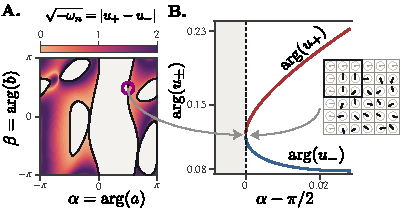
\includegraphics[width=\columnwidth]{Figure3.pdf}
\caption{\textbf{Ramified Hadamard completion at a branch collision.} \textbf{A.} Value of $\sqrt{-\omega_n} = \vert u_{+} - u_{-} \vert$ for varying ${\rm arg}(a)$ and ${\rm arg}(b)$ at fixed $c = {\rm i}$ and $d = d_{0} = \frac{1 + {\rm i}\xi_{0}}{1 - {\rm i}\xi_{0}}$, where $\xi_{0}$ is the unique real root of Eq.~\eqref{eq:ramification-seed-polynomial}. At the circled seed, the two branches of the quadratic in Eq.~(\ref{eq:horizontal-product-quadratic}) meet and $\omega_{n} = 0$ (black lines).  \textbf{B.} Arguments of the two roots of the relevant quadatics versus $\alpha$. They coalesce at $\alpha = \pi/2$ and $\beta = \pi/2$. The phase portrait of the ramified, product-regular completed Hadamard at this branch collision point is shown. Numerical diagnostics for this representative, reported in Supplemental Table~\ref{tab:supp-ramification-bounds}, distinguish it from the Karlsson, Tao, and four-$3\times3$-circulant-block
constructions.}
\label{fig:ramifiedHadamard}
\end{figure}

\paragraph*{A representative ramification seed.}
Let $\xi_0$ be the unique real root of
\begin{equation}
\begin{aligned}
P(\xi)={}&16\xi^7+120\xi^6+428\xi^5+952\xi^4\\
&+1363\xi^3+1231\xi^2+664\xi+176.
\end{aligned}
\label{eq:ramification-seed-polynomial}
\end{equation}
The Cayley seed
\begin{equation}
(a,b,c,d)=\left(\I,\I,\I,\frac{1+\I\xi_0}{1-\I\xi_0}\right),
\label{eq:ramification-cayley-seed}
\end{equation}
lies on the sheet-collision set $\omega_{\rm n}=0$, which is visualized in Fig.~\ref{fig:ramifiedHadamard}. Our high-precision numerics finds a product-regular completion and separates this seed from the Karlsson, Tao, and four-$3\times3$-circulant-block constructions. The numerical diagnostics are reported in Supplemental Table~\ref{tab:supp-ramification-bounds}.

\section{Proof of Sz\"oll\H{o}si's conjecture}
\label{sec:szollosi-conjecture}
%%%%%%%%%%%%%%%%%%%%%%%%%%%%%%%%%%%%
The purpose of this section is to prove Sz\"oll\H{o}si's Conjecture~4.2~\cite{Szollosi2012FourParameter}, clarifying the relationship between $G_6^{(4)}$, the notation he used for the generic family produced by his Construction~3.1, and $\FCAtlas_6^{\mathrm{fc}}$.

\begin{definition}[Sz\"oll\H{o}si's construction output]
\label{def:historical-G-output}
Following Sz\"oll\H{o}si, let $G_6^{(4)}$ denote the non-Karlsson, non-Tao classes returned by Steps~1--8 of his Construction~3.1 \cite{Szollosi2012FourParameter}. The definition includes every unimodular root and every finite common-root branch retained in Case~2 of his detailed construction. It excludes the identically vanishing fundamental-polynomial case for which that construction is declared to fail. Equivalently, by his Theorem~4.1, it is the output obtained from corners having finite nonempty
normalized invertible candidate sets. This is Sz\"oll\H{o}si's construction
output, not the output of our branch-complete procedure by definition. The
exclusion of Karlsson and Tao records his sector convention rather than an
obstruction inherent in fixed-corner dilation.
\end{definition}

At a product-regular corner, all elimination steps are reversible, so
Sz\"oll\H{o}si's Construction~3.1 and our quadratic--cubic
reconstruction produce the same candidate blocks and Hadamard
completions.


\begin{proposition}[Identification of Sz\"oll\H{o}si's sector]
\label{prop:historical-output-identification}
\begin{equation}
G_6^{(4)}
=
\FCAtlas_6^{\mathrm{fc}}\setminus
\bigl(\KK_6^{(3)}\cup\mathcal T_6\bigr).
\label{eq:historical-output-identification}
\end{equation}
\end{proposition}

\begin{proof}
Let $[H]\in G_6^{(4)}$. By
Definition~\ref{def:historical-G-output}, a representative of
$[H]$ is produced by Sz\"oll\H{o}si's Construction~3.1 from finite
normalized candidate sets. These candidates satisfy the parent
fixed-Gram equations, and the retained completion uses the same
forced-block formula and unimodularity tests as our branch-complete
procedure. Hence $[H]\in\FCAtlas_6^{\mathrm{fc}}$. Since
$G_6^{(4)}$ excludes the Karlsson and Tao sectors by definition,
this proves
\[
G_6^{(4)}
\subseteq
\FCAtlas_6^{\mathrm{fc}}\setminus
\bigl(\KK_6^{(3)}\cup\mathcal T_6\bigr).
\]

Conversely, let
\[
[H]\in
\FCAtlas_6^{\mathrm{fc}}\setminus
\bigl(\KK_6^{(3)}\cup\mathcal T_6\bigr).
\]
By the definition of $\FCAtlas_6^{\mathrm{fc}}$, some representative
of $[H]$ is recovered from a finite-corner witness.
Sz\"oll\H{o}si's Theorem~4.1 states that his Construction~3.1
exhausts all Hadamard completions at such a corner, including $H$.
Since $[H]$ is neither Karlsson nor Tao, it follows that
$[H]\in G_6^{(4)}$.
\end{proof}

\begin{corollary}[Sz\"oll\H{o}si's Conjecture~4.2]
\label{cor:szollosi-conjecture}
The three historical sectors form an exhaustive list:
\begin{equation}
\HH_6
=
G_6^{(4)}\cup\KK_6^{(3)}\cup\mathcal T_6,
\label{eq:szollosi-conjecture-list}
\end{equation}
and the three sectors are pairwise disjoint. Equivalently, every
class outside the Karlsson and Tao sectors is recovered by
Sz\"oll\H{o}si's Construction~3.1.
\end{corollary}

\begin{proof}
Corollary~\ref{cor:atlas-classification} gives
\[
\FCAtlas_6^{\mathrm{fc}}=\HH_6.
\]
Substitution into
Proposition~\ref{prop:historical-output-identification} yields
\[
G_6^{(4)}
=
\HH_6\setminus
\bigl(\KK_6^{(3)}\cup\mathcal T_6\bigr),
\]
which proves exhaustiveness and shows that $G_6^{(4)}$ is disjoint
from the other two sectors.

It remains only to separate Tao from Karlsson. Every cross ratio of
Tao's matrix is a cubic root of unity, whereas an $H_2$-reducible
matrix has a cross ratio equal to $-1$. Hence
$\mathcal T_6\cap\KK_6^{(3)}=\varnothing$.
\end{proof}

\section{Outlook}
\label{sec:outlook}
We have completed an explicit finite-corner classification of order-six complex Hadamard matrices. Specifically, we have proved that a representative of every equivalence class can be constructed from our branch-complete dilation procedure starting from four initial seeds in $\mathbb{T}^4$. This dilation procedure provides the missing step from Sz\"oll\H{o}si's Construction~3.1 and, as our procedure also covers the Karlsson and Tao sectors within the same framework, has allowed us to prove a stronger version of his Conjecture 4.2~\cite{Szollosi2012FourParameter}. 

Moreover, outside the Tao sector and the sector represented by a single explicit Karlsson matrix, we show that every equivalence class admits a \textit{product-regular} witness. In this case, the branch-complete dilation procedure simplifies to solving only two quadratic and two cubic equations, whose discriminant provides the geometric criterion for product regularity.

A direct experimental application of this work is multiphoton interference in balanced six-mode networks. After normalization, every order-six Hadamard matrix is a lossless six-port unitary with uniform single-particle probabilities, while its internal phases remain observable in multiparticle correlations. Such transformations are already realized in programmable photonic circuits, where two-photon experiments distinguish networks that are identical at the single-particle level~\cite{Carolan2015Universal,Laing2012BerryPhase,Tichy2010ZeroTransmission,Crespi2015Sylvester,Crespi2016FFT,Shchesnovich2015Partial}. Our results supply a complete, finite-chart design space for these balanced six-port transformations, extending searches for suppression laws and phase-sensitive interference signatures beyond selected families. The same Hadamard ingredient recurs as a coherence-generating gate~\cite{Yao2016MaximalCoherence} and as a building block of dual-unitary circuits, a standard testbed for entanglement growth and thermalization~\cite{Gutkin2020DualUnitary,Claeys2022StateDesigns}. In each setting our theorem classifies the Hadamard ingredient, while device-specific constraints remain explicit conditions on this complete space.

The classification does not settle the problem of mutually unbiased bases in $\mathbb C^6$, but it removes the need to search over an unclassified set of Hadamard matrices. After fixing one basis as standard, every transition matrix to a second unbiased basis satisfies $[\sqrt6\,U]\in\FCAtlas_6^{\mathrm{fc}}$.
With three or more bases, each basis is shared by several transition matrices at once, so the relabelings and phase choices used to reach standard form cannot be applied independently to each matrix: fixing one shared basis constrains every matrix built from it. The remaining task is to impose these joint compatibility conditions directly on the classified space constructed here~\cite{WoottersFields1989,BengtssonEtAl2007,HorodeckiRudnickiZyczkowski2022,McNultyWeigert2026,MatolcsiEtAl2026MUBTriplets}. 
This also gives a controlled domain for exact or certified searches in quantum-state determination, cryptography, and related measurement-design
problems~\cite{WoottersFields1989,Cerf2002,Englert2001,Aravind2003}. An important structural question is whether analogous finite-corner arguments extend to complex Hadamards in higher orders. 



%%%%%%%%%%%%%%%%%%%%%%%%%%%%%%%%%%%%%%%%%%%%%%%%%%
\section*{Acknowledgements}
The authors thank Andy Millis and Uli Schollwöck for helpful discussions on this manuscript.
We thank Gavin Crooks for suggesting that the structural inputs be derived internally in the Lean formalization.
M.C.W. acknowledges the hospitality of the Center for Computational Quantum Physics at the Flatiron Institute. The Flatiron Institute is a division of the Simons Foundation.

OpenAI's ChatGPT Sol 5.6 Pro and Codex 5.6 Sol and Claude's Opus 5.0 were used interactively in the development of this work. The LLMs assisted in proposing and testing proof strategies, searching for gaps and possible counterexamples, checking intermediate algebra, drafting and debugging symbolic and formal-verification code, and revising the manuscript. 
%
The authors specified the definitions and target statements, supplied and checked the relevant literature, selected the proof strategies, reviewed proposed arguments and counterexamples, and decided which derivations and computations to retain.
%
Several model-generated proposals were found to be incomplete or incorrect and were either discarded or repaired. 

The authors independently checked all retained LLM-assisted material and verified the computer-assisted claims described in the Supplemental Material. The authors take full responsibility for the mathematical content and presentation of this work.

%%%%%%%%%%%%%%%%%%%%%%%%%%%%%%%%%%%%%%%%%%%%%%%%%%
\section*{Data availability}
No external datasets were used. The accompanying repository at \url{github.com/mateocardeneswuttig/all_hadamard_matrices_in_dimension_six} contains the Lean~4 formalization and its pinned dependencies~\cite{CardenesWuttig2026HadamardRepository}, together with
the exact and interval certificates supporting the computer-assisted proofs for the results in
in Sec.~IV~\cite{CardenesWuttig2026HadamardRepository}. The public entry point \path{Hadamard6/PaperTheorem.lean} verifies Theorem~\ref{thm:classification} and Corollary~\ref{cor:atlas-classification}, including the two structural results stated in Proposition~\ref{prop:publishedinputs}. The \path{certificates/} directory contains the certificates, and \path{certificates/PAPER_CLAIM_AUDIT.md} maps each computer-assisted claim to its verifier.

%%%%%%%%%%%%%%%%%%%%%%%%%%%%%%%%%%%%%%%%%%%%%%%%%%
\bibliography{ref}
\fi
